\documentclass[11pt]{article}
\usepackage[margin=1in]{geometry}
\usepackage{biblatex}
\bibliography{main} 
\addbibresource{main.bib}
\usepackage{amsmath}
\usepackage{listings}
\usepackage{graphicx}
\usepackage{subfig}
\usepackage{caption}
\usepackage{float}
\usepackage{todonotes}
\usepackage[export]{adjustbox}
\usepackage{wrapfig}
\usepackage{sidecap}

\title{Machine Learning Review}
\author{Francesco Saverio Zuppichini}
\begin{document}
\maketitle
The aim of this report is to summarise the topics threaded in my Machine Learning class at USI.
\section{History of Machine Learning}
\todo[inline]{Write something about the history of ML}

\section{Gradient Descend}
The gradient descend is an iterative optimisation algorithm that follows the direction of the negative gradient in order to minimised an objective function. It can be effectively used as Learning Algorithm because it reduces the error function, Equation \ref{eq: MSE_perceptron}, and adjusts the weights properly. Equation \ref{eq: GD} shows the generic update rule.
\begin{equation}
	w_{k + 1} = w_k - \eta \nabla E(w_k)
	\label{eq: gradient_descent}
\end{equation}
Where $\eta$ is the step size, also called \textbf{learning rate} in Machine Learning. This parameter influences the behaviour of gradient descent, a small number can lead to local minimum, while a bigger learning rate could "over-shoot" and decreasing the converge ration. Later in this project you will see how a wrong $\eta$ can strongly change the output of a Neural Network.

For this reasons, numerous improvements have been proposed to avoid local minima and increase its convergence ration, some of them are: Conjugate Gradient and Momentum.
\subsection{Loss Functions}
In order to apply gradient descend we need a loss function to minimise, usually they are divided by problem type;

\begin{itemize}
	\item \textbf{For Regression} \\
	Mean Square Error: \\
	\begin{equation}
	E = \frac{1}{N}\sum_{i=1}^N(\underbrace{y_i}_{\text{predicted}} - \underbrace{t_1}_{\text{actual}})^2
	\label{eq: MSE}	
	\end{equation}
	\item \textbf{For Classification} \\
	SoftMax Function:
	\begin{equation}
	y_j = \frac{e^{x^Tw_j}}{\sum_{k = 1}^K e^{x^Tw_k}}
	\label{eq: soft_max}	
	\end{equation}
	with negative log likelihood:\\
	\begin{equation}
	- \sum_{i = 1}^K t_ilog(y_i)
	\label{eq: log_like}
	\end{equation}
	
\end{itemize}
\section{Perceptron}
\subsection{Definition}
The \textbf{Perceptron} is binary  \textbf{linear classifier} algorithm used in \textbf{supervised learning}. It can be seen as the most basic form of Neural Network. Equation \ref{eq: perceptron} defines the its output.
\begin{equation}
f(x) \left \{ 
 \begin{tabular}{lcc}
  1 \quad \text{if} w \cdot x + b \ge  0 & & \\ 
  0 \quad \text{otherwise} &  & 
  \end{tabular}	
  \label{eq: perceptron}
\end{equation}
Given a training set $D = \{ (x_1,t_1}, ... , (x_n,t_i) \}$, $x_i \in X$ and $t_i \in Y$ denotes the input vector and the target vector respectively. We express $y = f(x)$ as the output of the algorithm, $w$ the weight and $b$ the bias. At each iteration the error is calculated using the Mean Square Error, defined in equation \ref{eq: MSE}
%\begin{equation}
%	E(w) = \frac{1}{N}\sum_{i = 1}^N(\underbrace{y(x_i,w_i)}_{\text{predicted}} - \underbrace{t_i}_{\text{actual}})^2)
%	\label{eq: MSE_perceptron}
%\end{equation}
The algorithm uses stochastic \textbf{Gradient Descent} in order to update the weight at each iteration using the formula defined in Equation \ref{eq: gradient_descent}.
 
\begin{equation}
	\frac{\partial E}{\partial w_k} = y - t
\end{equation}
\section{Neural Network}
A \textbf{Neural Network} is a universal function approximation. It is a nested composite functions like $f(g((h...)))$. In its simplest representation, an FeedForward Neural Network, it is composed by a \textbf{input layer}, an \textbf{hidden layer} and an \textbf{output layer}. The size of the hidden layer is usually refers as the \textbf{deepth} of the network.
\subsection{Forward pass}
In order to get the prediction out of our network we need to calculate the compute the activation at each layer $l$.
Equation \ref{eq:forward_pass} shows the activation $a$ of layer $l$ for the $j$-th neuron on that layer.

\begin{equation}
\label{eq:forward_pass}
a^l_j = \sigma(\sum_k w^l_{jk}a^{l-1}_k + b^l_j)
\end{equation}

Where $w^l_{jk}$ is the connection from neuron $k$ in the $l-1$ layer to $j$, $a^{l-1}$ is the activation of the previous layer and $b^l_j$ is the bias of $j$-th neuron in the $l$ layer. With this in mind, we can rewrite \ref{eq:forward_pass_vectorized} in a efficient vectorised form
\begin{equation}
a^l = \sigma(W^la^{l-1} + b^l)
\label{eq:forward_pass_vectorized}

\end{equation}

\subsection{Delta rules}
In a Neural Network the weights are iteratively changed in order to decrease the cost function, called $E$. We want to find out how much they should be updated, in order to do so we need the output error at each layer. Equation \ref{eq: deltaRule_1} defines $\delta^l_j$ as the \textbf{output error} of neuron $j$ in layer $l$
\begin{equation}
	\delta^l_j = \frac{\partial E}{\partial z^l_j}
	\label{eq: deltaRule_1}
\end{equation}
Strictly speaking, $\delta^l_j$, is how much the error function changes by changing the weighted input on that layer. Applying the chain rule, Equation \ref{eq: deltaRule_1} becomes:
\begin{equation}
\delta^l_j = \frac{\partial E}{\partial a^l_j} \frac{\partial a^l_j}{\partial z^l_j}
\label{eq:deltaRule_2}
\end{equation}
By knowing that $a^l_j = \sigma(z^l_j)$, Equation \ref{eq:deltaRule_2} can be expressed as:
\begin{equation}
\delta^l_j = \frac{\partial E}{\partial a^l_j} \sigma'(z^l_j)
\label{eq:deltaRule}	
\end{equation}

Also, delta at layer $l$ can be expressed by using the next $l+1$-th delta. Equation \ref{eq: delta_on_delta} shows the new rule.
\begin{equation}
\delta^l = (W^{l+1}\delta^{l+1}) * a^l
\label{eq: delta_on_delta}
\end{equation}
\subsection{Back Propagation}
The \textbf{Back Propagation} algorithm defines an efficient and interactive method to calculate the gradient at each layer. We want to compute $\frac{\partial E}{\partial w^l_{jk}}$, by applying the delta rule: 
\begin{equation}
\frac{\partial E}{\partial w^l_{jk}} = \frac{\partial E}{\partial z^l_j}\frac{\partial z^l_j}{\partial w^l_{jk}} =	
\frac{\partial E}{\partial a^l_j}\frac{\partial a^l_j}{\partial z^l_{j}}
\end{equation}
After some calculation we derive Equation \ref{eq: back_propagation} that shows the partial derivative of the error function with respect to the weight of the $l$-th layer for the $j$-th neuron using the error output in that layer.
\begin{equation}
\frac{\partial E}{\partial w^l_{jk}} = a^{l-1}_k \delta^l_j
\label{eq: back_propagation}
\end{equation}  
While \ref{eq: back_propagation_bias} shows how to calculate the derivative of the error with respect to the bias.
\begin{equation}
\frac{\partial E}{\partial b^l_j} = \delta^l_j
\label{eq: back_propagation_bias}
\end{equation}
We know from Equation \ref{eq: delta_on_delta}, $\delta^l$ can be calculated used the $l+1$-th layer's information, this is why is called \emph{back} propagation since we used the last layer information in order to, each time, find out the next layer's delta until we reach the input layer.
After computed the gradient with respect to each weight and bias the can use gradient descent described in section 2 in order to update each one of them according to Equation \ref{eq: gradient_descent}.
\section{Convolutional Neural Network}
Convolutional neural networks are neural network that uses a \textbf{convolutional} operation at place in at least one layer. They are used for processing grid-like data, such as time-series, a 1D grid and images, 2D grid. Figure \ref{fig: cnn} shows a the generic architecture for a CNN.
\begin{figure}[H]
\centering
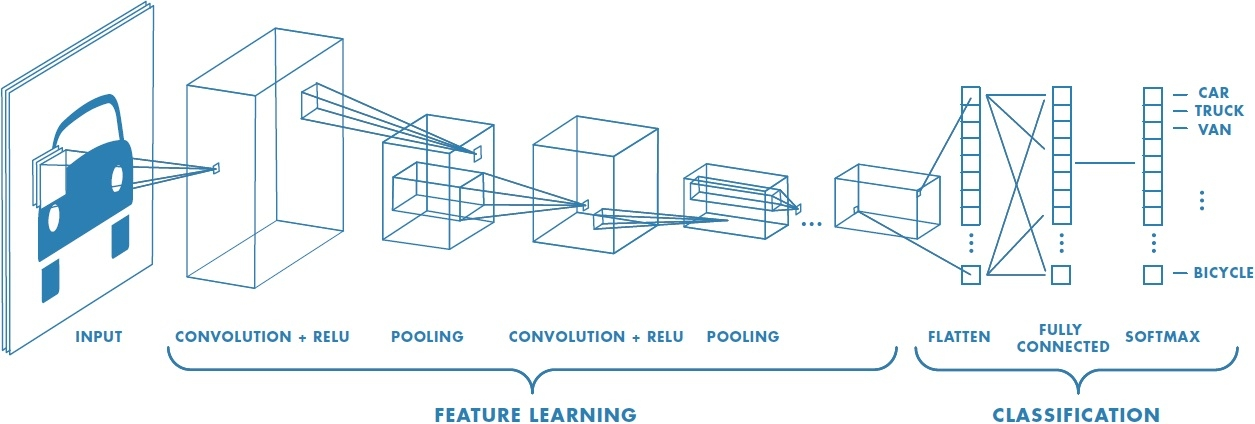
\includegraphics[scale=0.35]{images/cnn}
\caption{}
\label{fig: cnn}	
\end{figure}
\subsection{Notation}
We express an Image as a function $f: \mathbb{Z}^2 \rightarrow \mathbb{R}^c$, where $c$ is the number of channel, in a color image there are three (rgb). A Windows is a subset of the image domain, $W \in \matbb{Z}^2$, that corresponds to a rectangle inside the image.
\subsection{Convolutional Layer}
As in a hidden layer, a Convolutional layer is formed by $n$ neurons. The difference is that they are not necessarily connect to the activations of the neurons in the previous layer, but only in a particular window.
The architecture is composed as following:
\begin{itemize}
	\item A input $[w*h*c]$ holds the an image
	\item A convolutional layer computes the output of its neurons that are connected to some window in the input, each computes the dot product between its weight and the region they are connected to. Each neuron apply a filter, usually of size $3x3$ or $5x5$.
	\item A rectifier function, RELU $max(0,x)$, is applied in order set to zero the not discovered features.
	\item A max-pool layer perform a downsampling operation, storing only the most relevant feature (the biggest number) in a little window size (usually $2x2$). Figure \ref{fig: pool} shows a visual representation of this operation
\begin{figure}[H]
\centering
	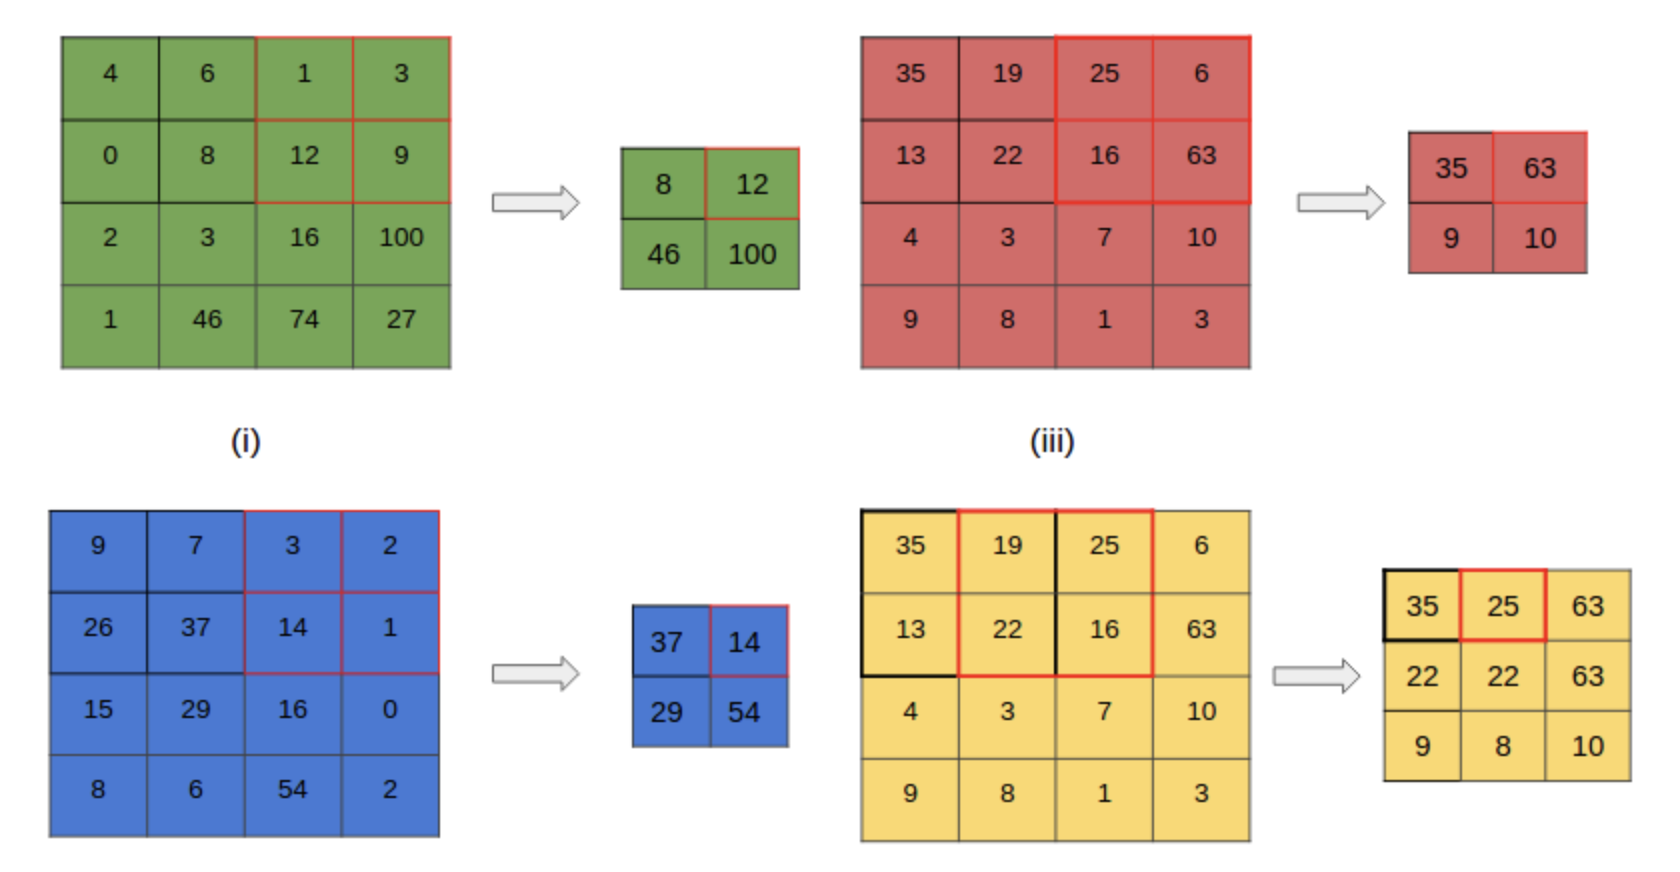
\includegraphics[scale=0.5]{images/pool}
	\caption{}
	\label{fig: pool}
\end{figure}
	\item A fully connected layer computes the class scores using softmax, Equation \ref{eq: soft_max} in order to equally distribute the probabilities.
\end{itemize}
After each CONV $\rightarrow$ RELU $\rightarrow$ POOL layer the network learn more complex pattern each time, Figure \ref{fig: cnn_faces} shows an example where in the first layer the network can only recognise little lines and in the last one it is able to merge all the previous information and classify very complex pattern such as a human face
\begin{figure}[H]
\centering
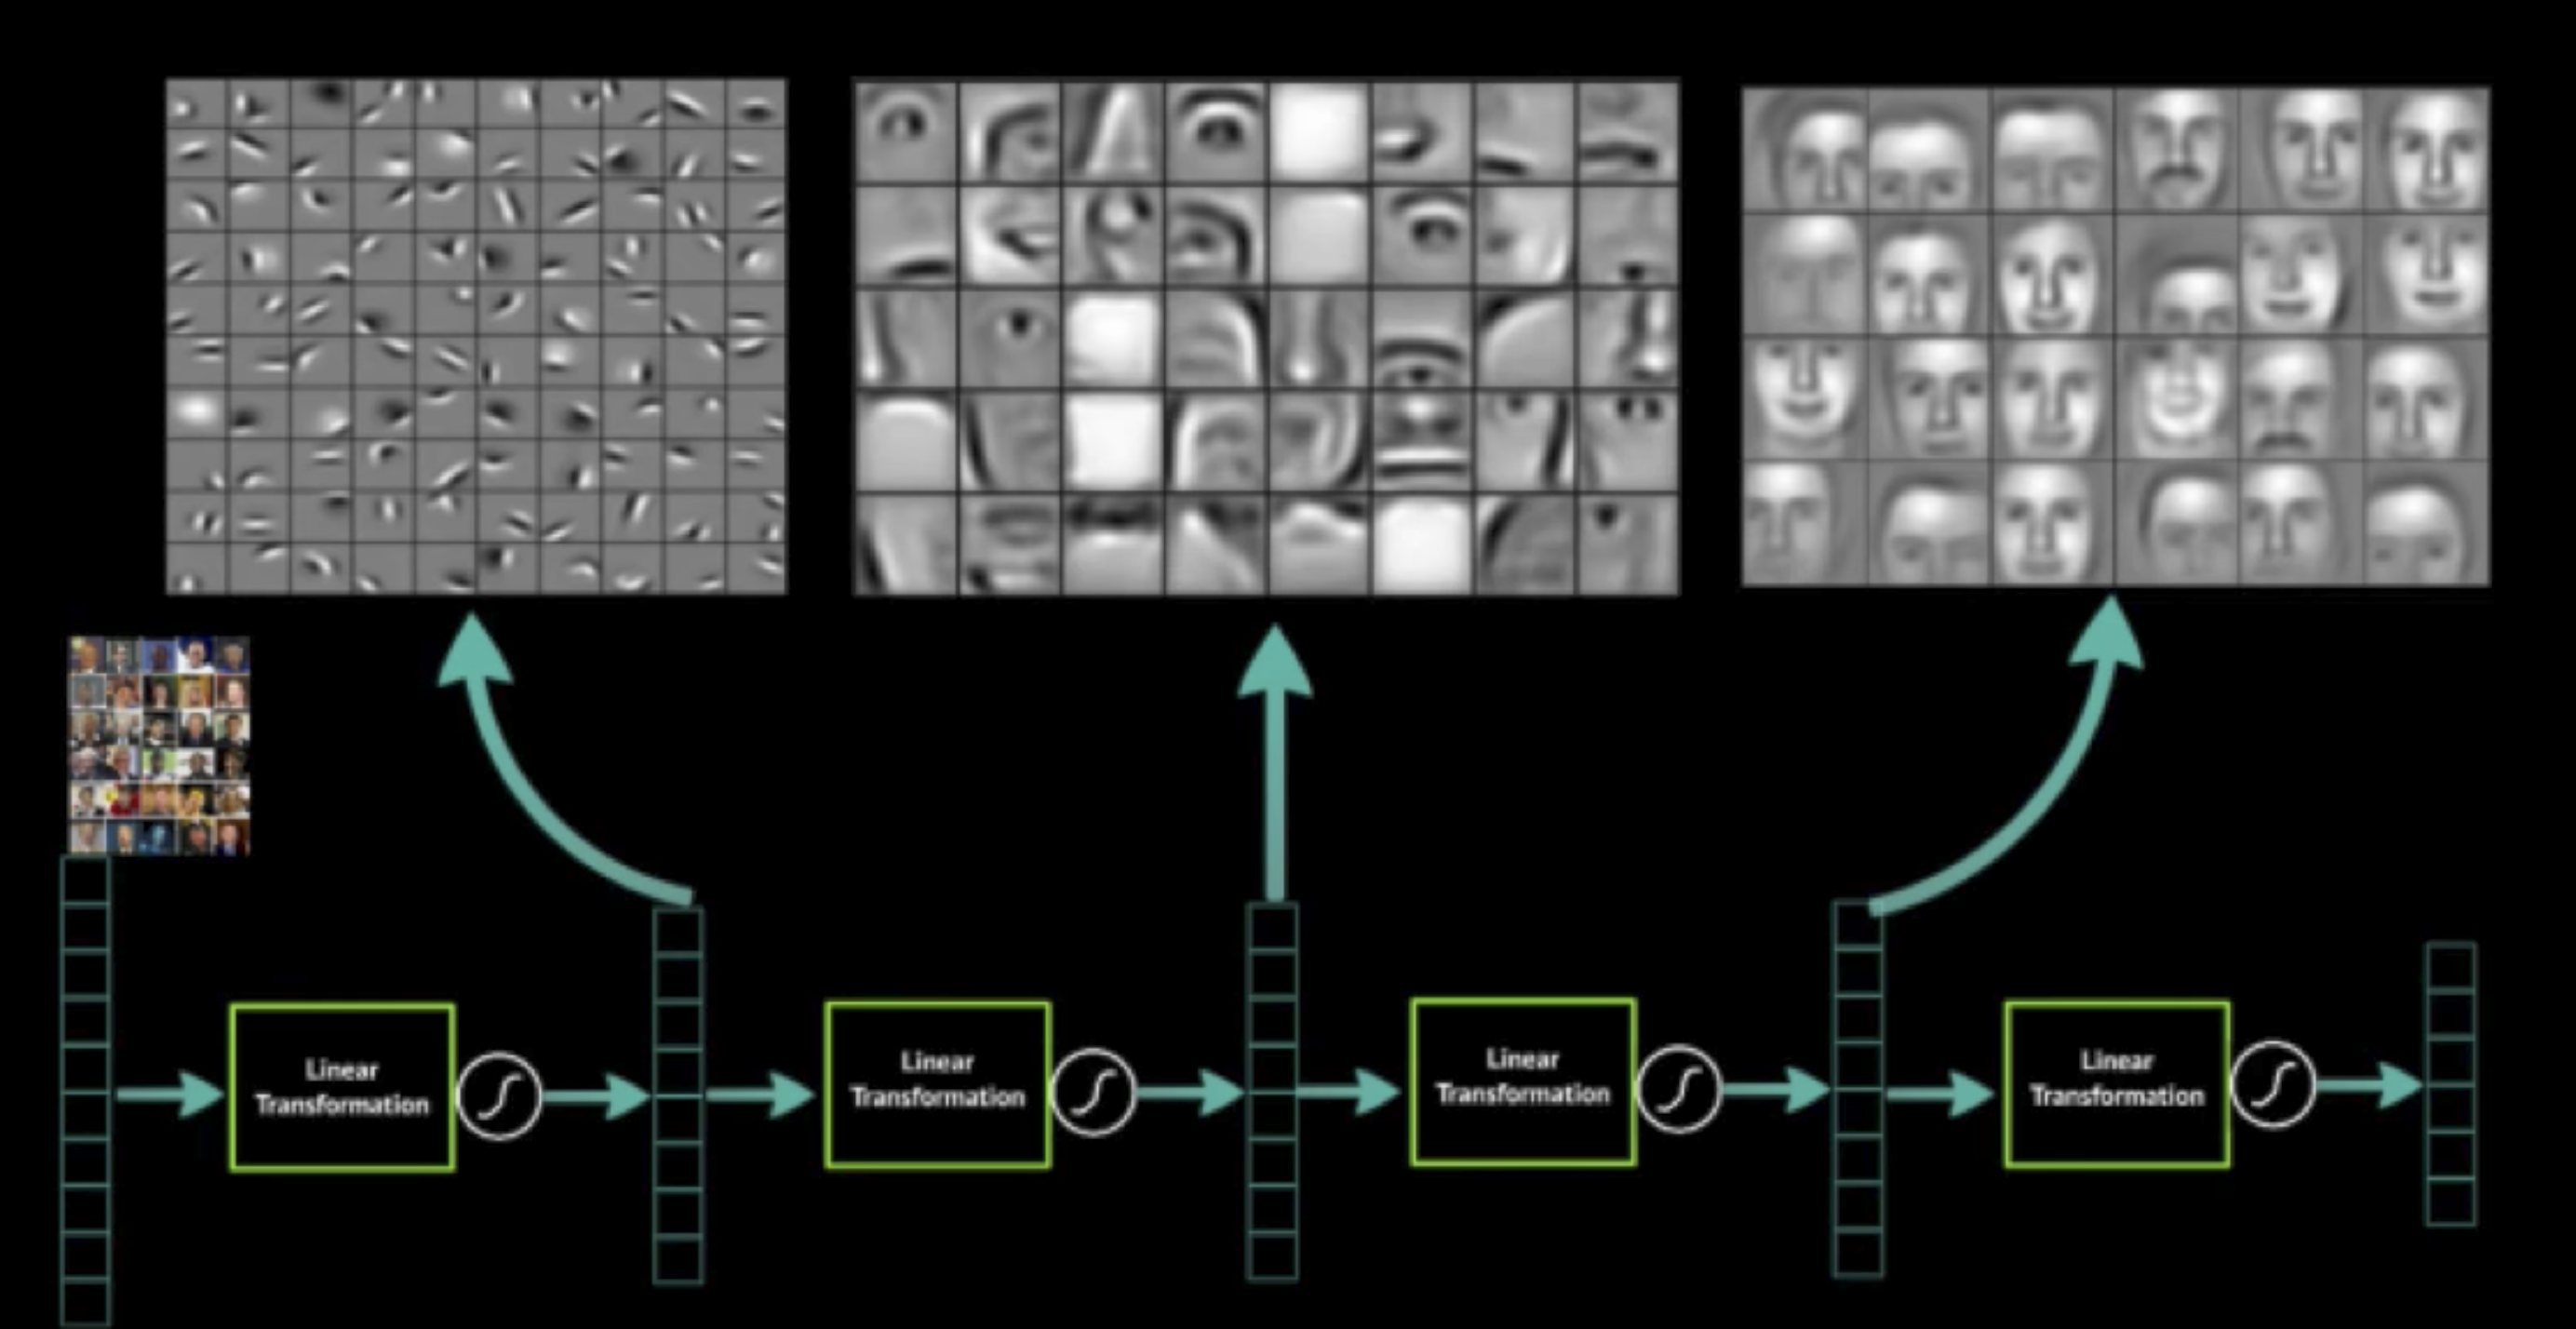
\includegraphics[scale=0.35]{images/cnn_faces}
\caption{}
\label{fig: cnn_faces}	
\end{figure}
The \textbf{pooling} layer is used to get out from the convolutional layer only the most important features, in order to do so usually a $2X2$ matrix is 
\section{Recurrent Neural Network}
\subsection{Definition}
A Recurrent Neural Networks can remember past decision by taking as input not only the current input but also the last time state. For this reason it is said that a RNN has \textbf{memory}. Figure \ref{fig: RNN} shows a classic representation. Usually, a RNN is represented unfolded to highlight the time dependencies. Due to its ability to remember it mostly used in text and speech recognition.
\begin{figure}[h]
\centering
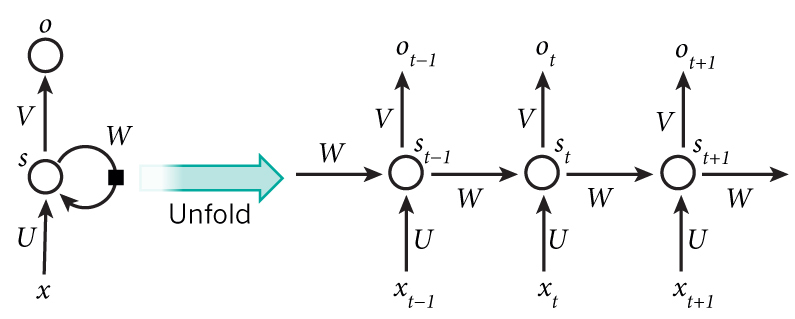
\includegraphics[scale=0.2]{images/rnn}	
\caption{Fold and Unfold representation of a RNN}
\label{fig: RNN}
\end{figure}

Very similar to a feedforward network, Equation \ref{eq: output_rnn} shows the weighted output at layer $j$. The first term on the right-hand is just the feedforward's weighted output, while the second term is the time-dependent term. Matrix $\omega$ is a hidden-state-to-hidden-state matrix. Basically, we are adding previous informations to our new state at time $t$.
\begin{equation}
z[t]^l = (W^la[t]^{l -1}+ b^l_j) + (\omega^l a[t-1]^{l-1})
\label{eq: output_rnn}	
\end{equation}
Equation \ref{eq: activation_rnn} shows the activation of layer $j$ at time $t$.
\begin{equation}
a[t]^l	= \sigma(z[t]^l)
\label{eq: activation_rnn}
\end{equation}
While Equation \ref{eq: rnn_weigt_update} shows the updating rule for the weight $w^l$
\begin{equation}
\begin{matrix}
\frac{\partial E}{\partial w^[T]l_{jk}} =\sum^T_{t=0} \frac{\partial E}{\partial z[t]^l_j}	\\ 
\\
\frac{\partial E}{\partial w^[T]l_{jk}} = \sum^T_{t=0} a[t]^{l-1}_k \delta[t]^l_j	
\end{matrix}
\label{eq: rnn_weigt_update}
\end{equation}
\subsection{Loss}
Usually in a RNN the loss used function is the \textbf{cross-entropy loss}. For example, suppose we have $K$ samples with each sample labeled by $i, ... K$. The loss function is then given by Equation \ref{eq: log_like}
%\begin{equation}
%E = -\frac{1}{N}\sum^N_{n=1}	t_n \log y_n
%\label{eq: cross_entropy}	
%\end{equation}

 
\subsection{Vanishing Gradient Problem}
Since the network layers and time steps are related to each other through multiplication, the gradient becomes smaller and smaller at each $t$. Figure \ref{fig: sigmoid_over_time} shows the effect of applying $sigmoid$ function over time. The data is flatted more and more at each step and therefore the slope will $\rightarrow 0$.
\begin{figure}[H]
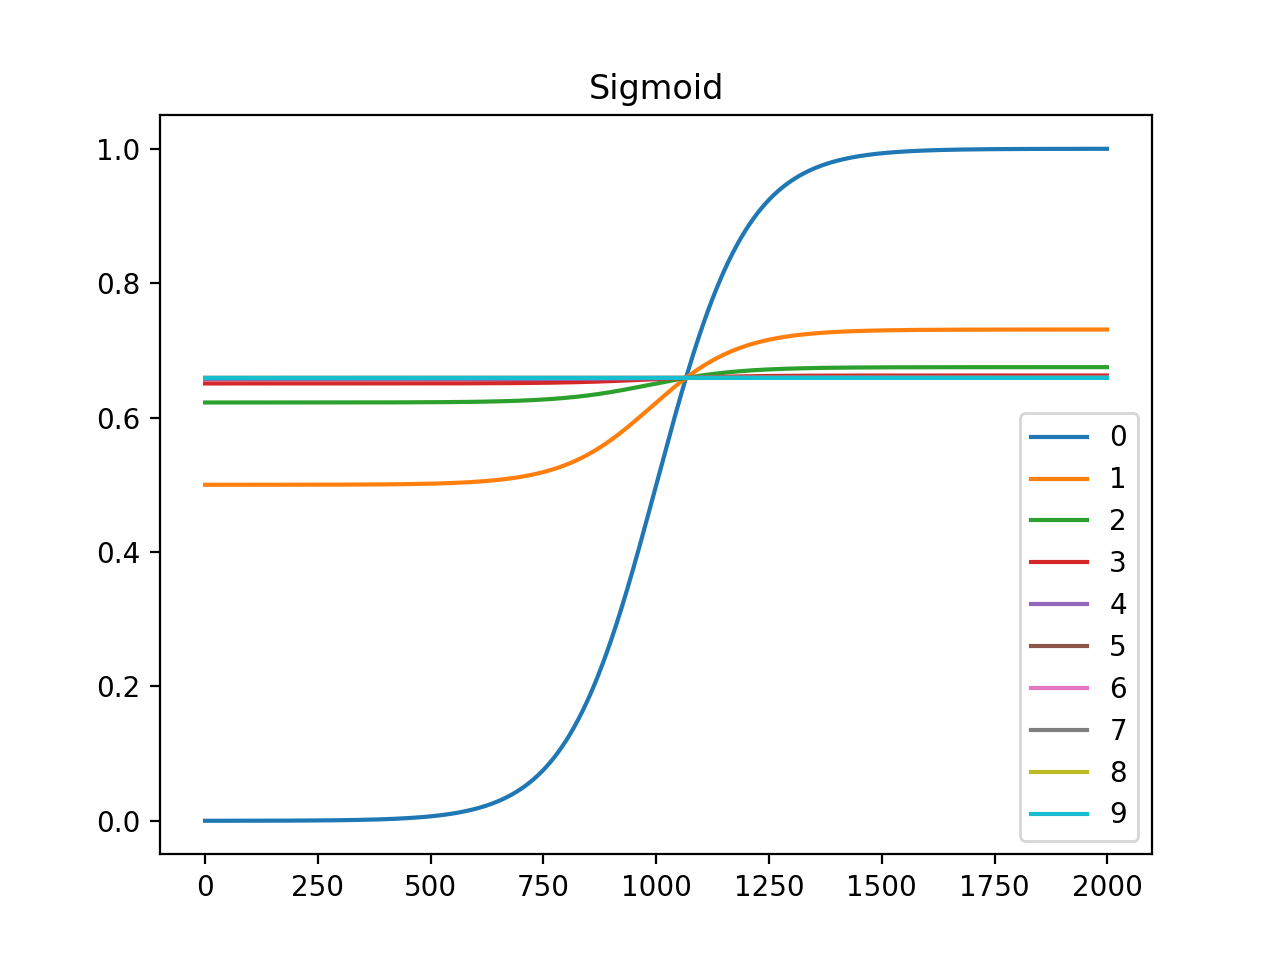
\includegraphics[scale=0.5]{images/sigmoid_gradient_vanish}
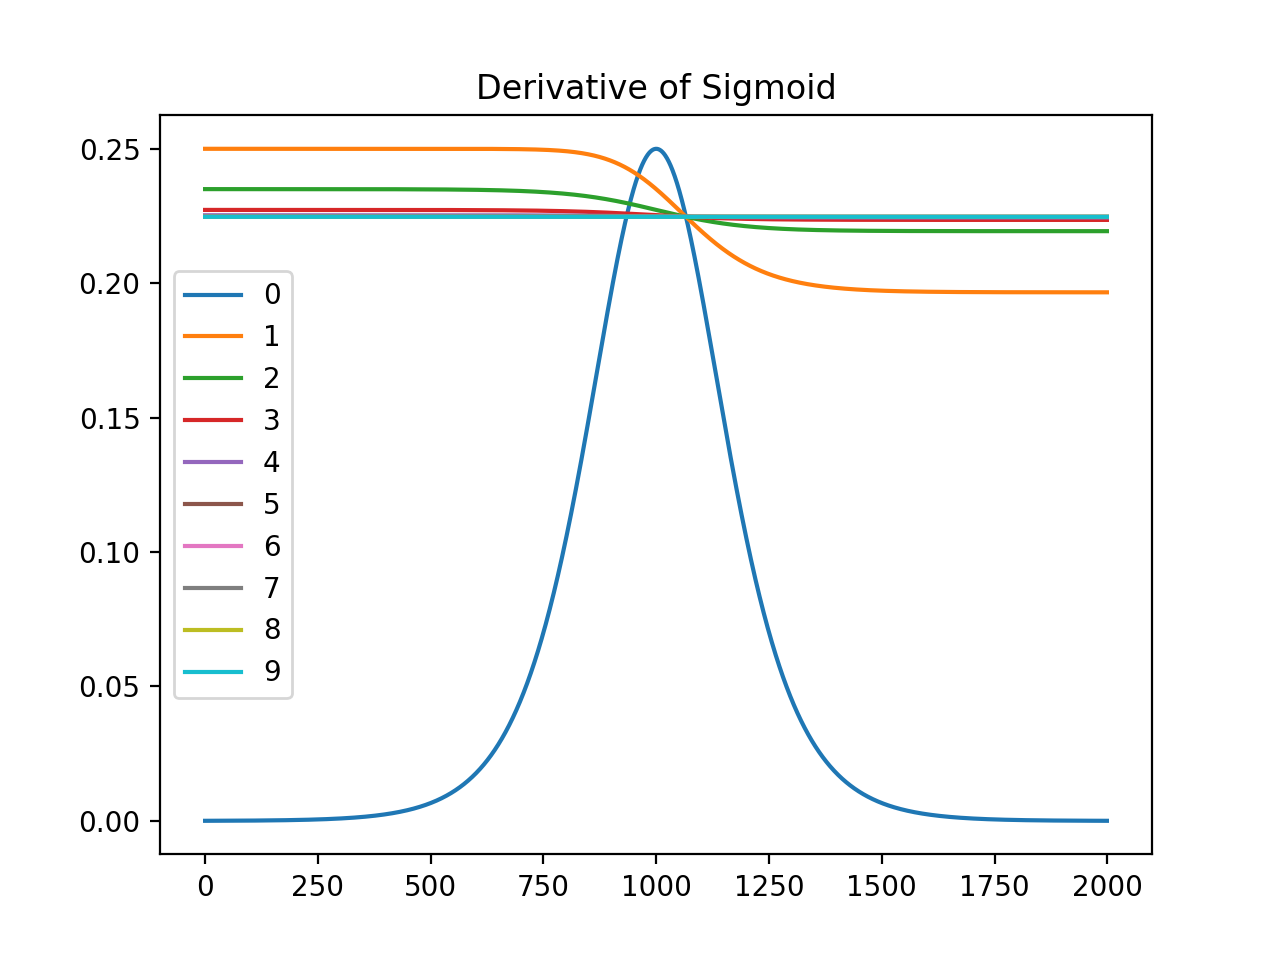
\includegraphics[scale=0.5]{images/sigmoid_gradient_vanish_derivative}
\caption{Sigmoid and its derivative over time}
\label{fig: sigmoid_over_time}	
\end{figure}
Since gradient expresses the change in all weights with respected to the error, without nothing it we cannot adjust properly the network.

\section{Long Short Term Memory}
\subsection{Definition}
The Long Short Term Memory networks, or just \textbf{LSTM}, are a special type of RNN capable of learning long-term
dependencies. They were introduced by Juergen Schmidhuber in order to solve the vanish gradient problem. They are composed by LSTM cell, 
Figure \ref{fig: unrolled_LSTM} shows a unrolled representation.
\begin{figure}[H]
\centering
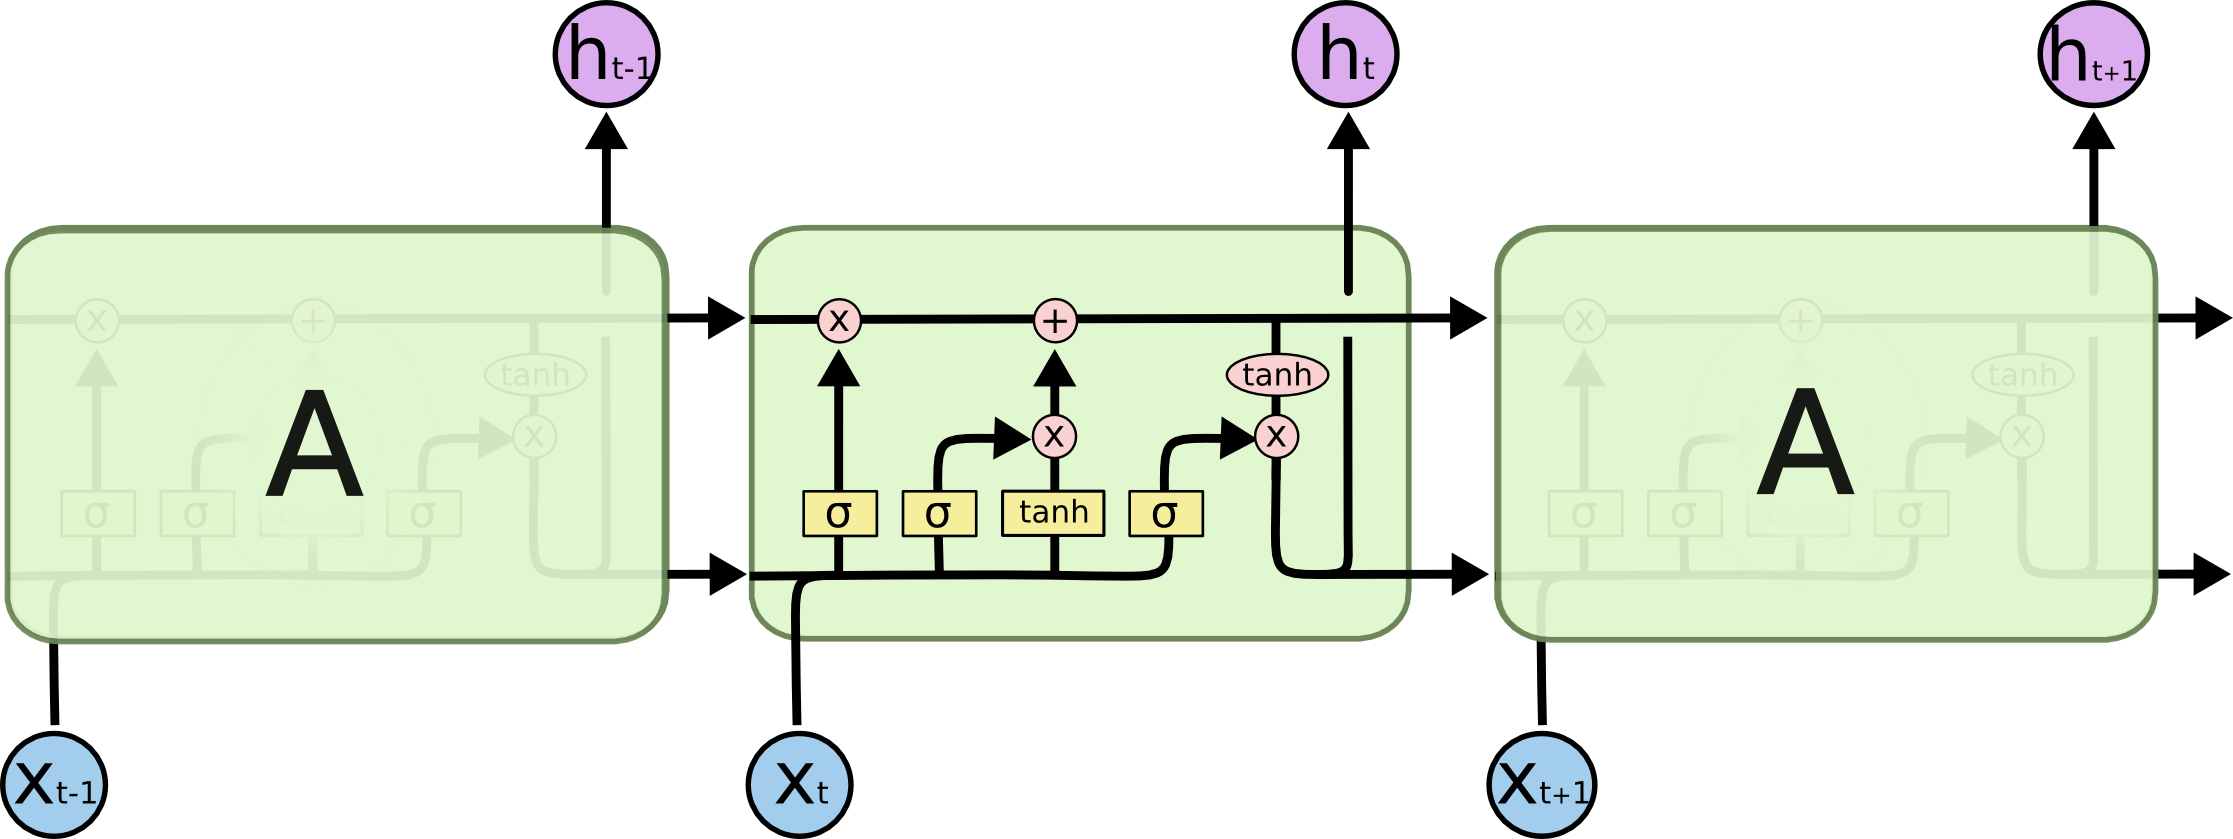
\includegraphics[scale=0.5]{./images/LSTM3-chain.png}	
\caption{An unrolled LSTM}
\label{fig: unrolled_LSTM}
\end{figure}
Each cell is composed by 3 gate: \textbf{forget} gate ($f_t$), \textbf{input} gate $i_t$ and \textbf{output} gate ($o_t$). It takes as 
input the previous output $h_{t - 1}$ and the old cell state $C_{t-1}$, it outputs the next prediction and state, $h_{t}$ and $C_t$. The cell
computes four basic operations:  
% \begin{enumerate}
	% \item
\begin{enumerate}
	\item Forget Gate \\ 
		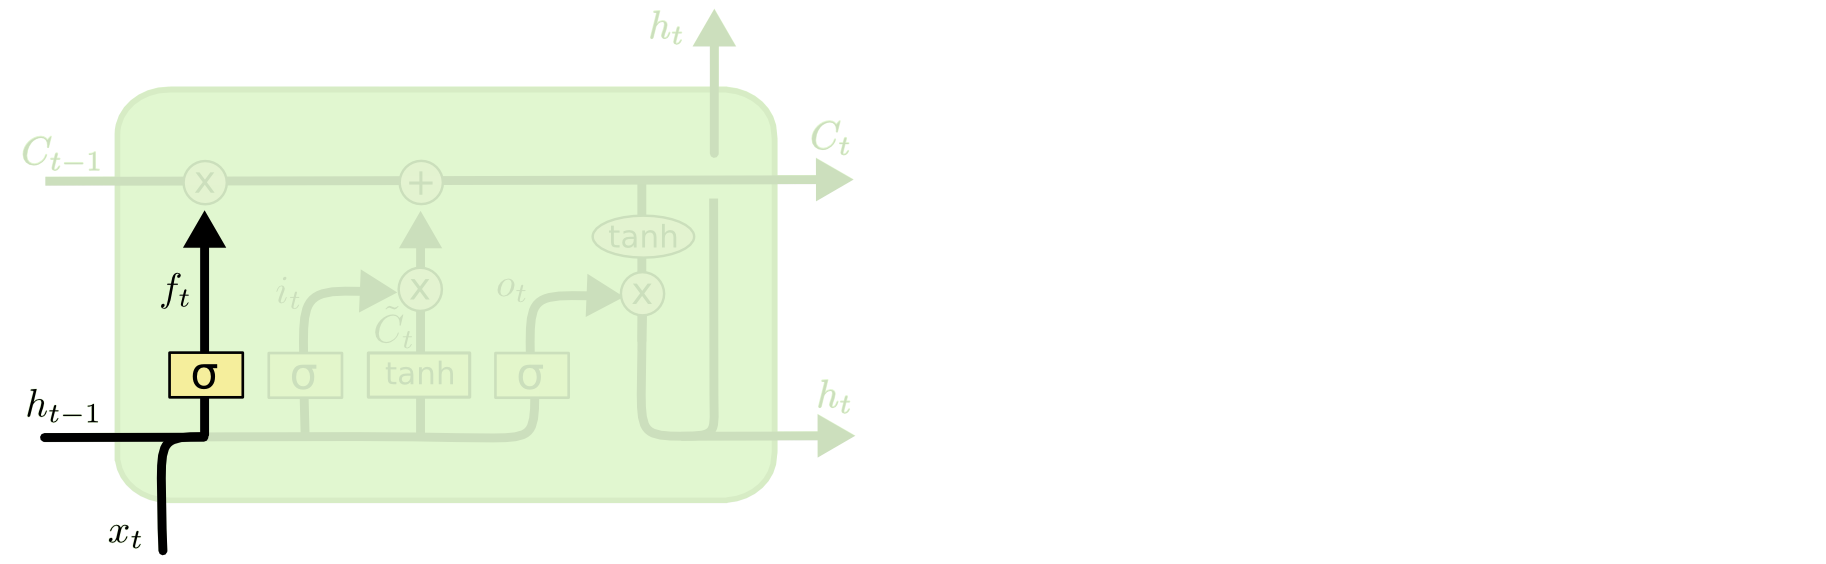
\includegraphics[scale=0.5]{./images/LSTM3-focus-f.png}
\item Input Gate \\
 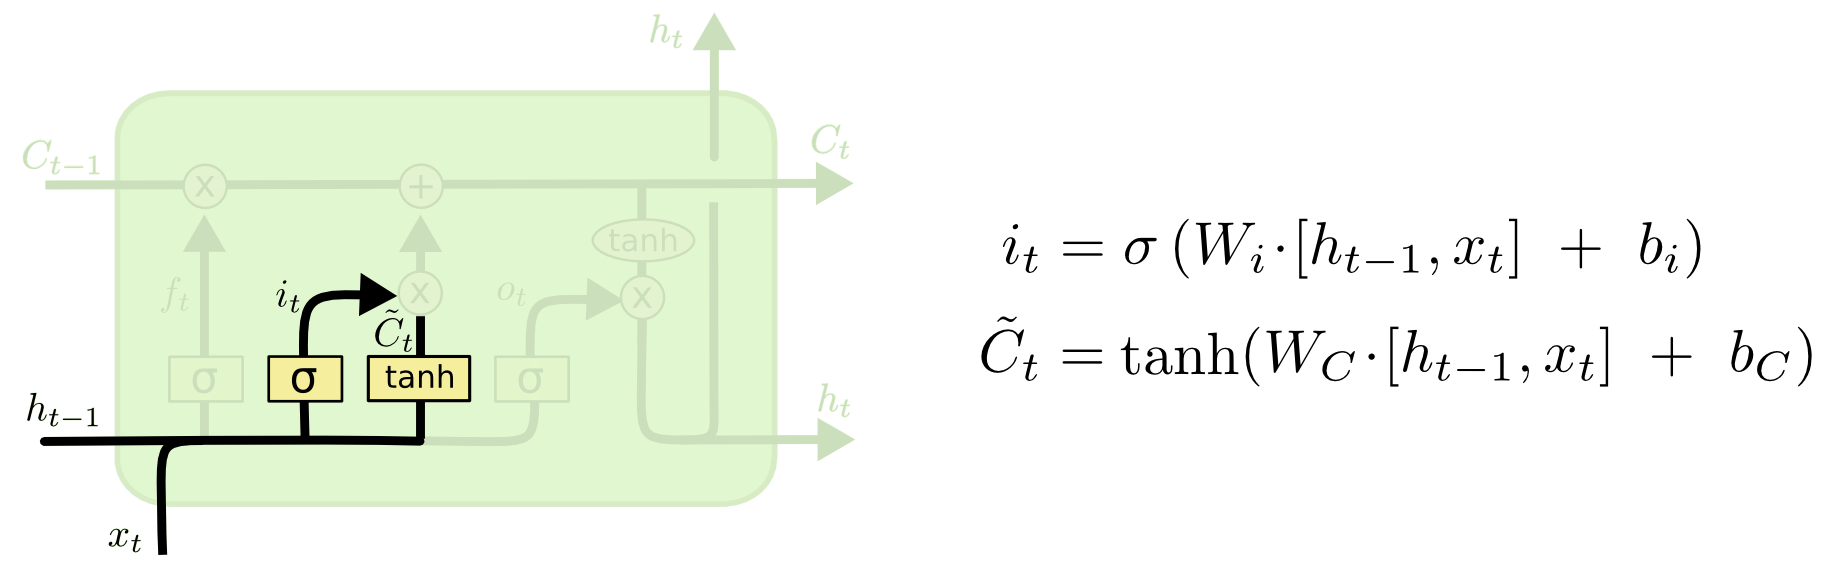
\includegraphics[scale=0.5]{./images/LSTM3-focus-i.png}
\item Update Cell State \\
		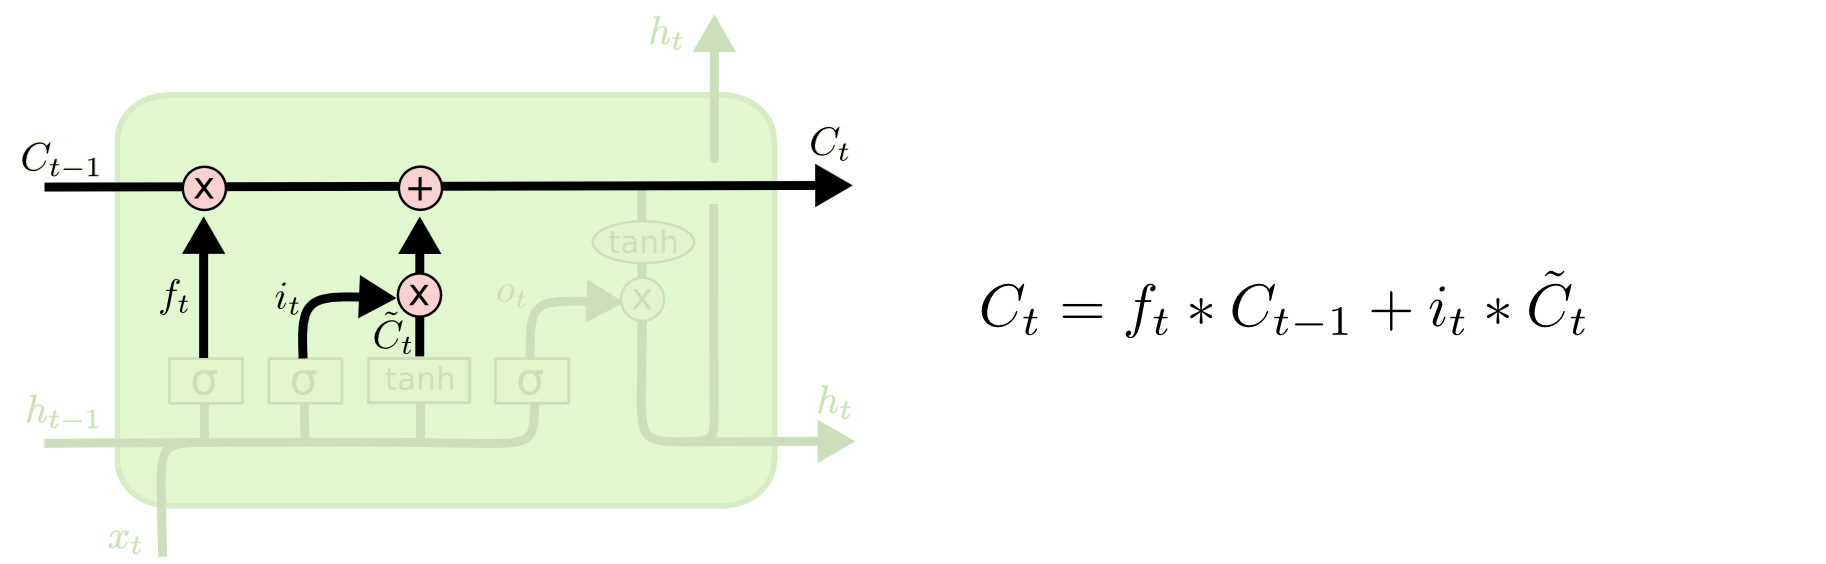
\includegraphics[scale=0.5]{./images/LSTM3-focus-C.png}
\item Output Gate	\\
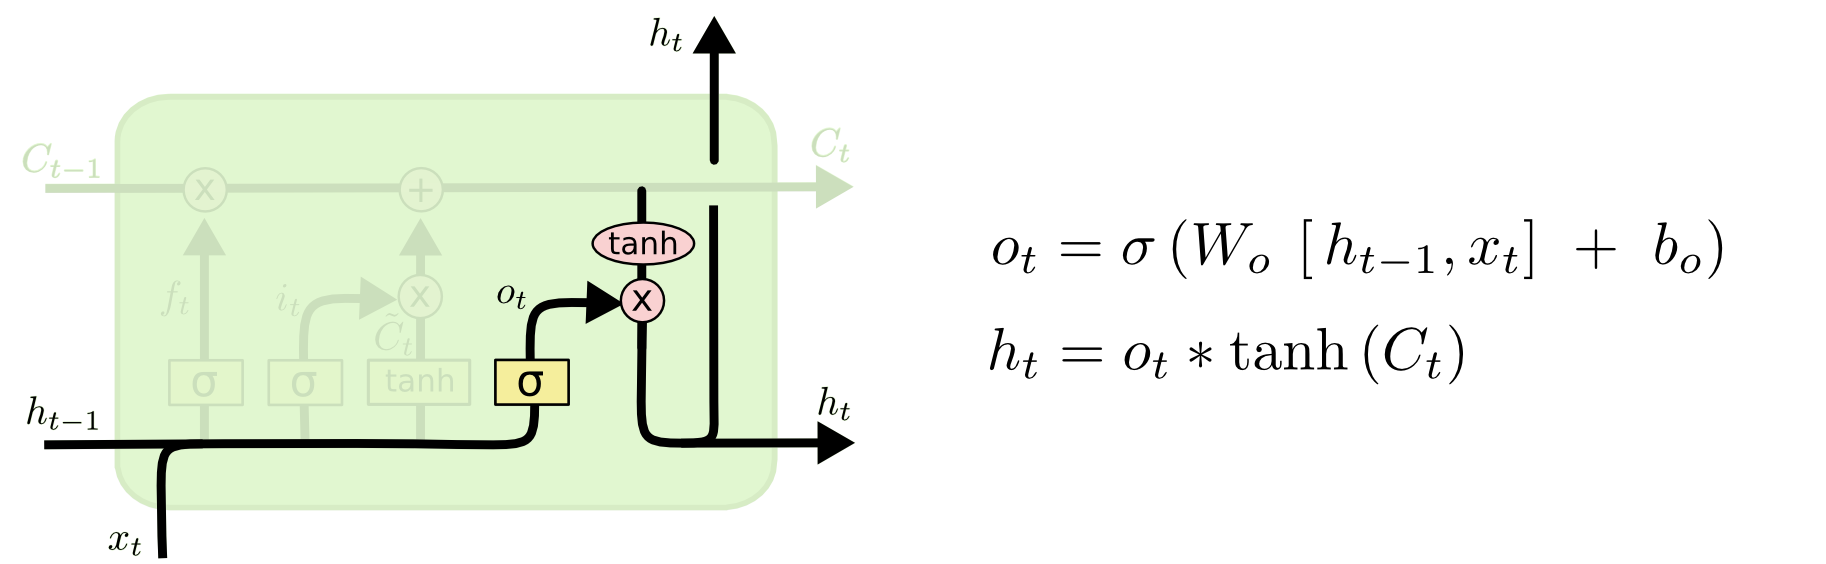
\includegraphics[scale=0.5]{./images/LSTM3-focus-o.png}
\end{enumerate}
	
% \end{enumerate}
\section{Support Vector Machine}

A Support Vector Machine maps the input space to a high dimensional space, called \emph{feature space}, using a set of non linear function, 
called the \emph{feature vector}, defined as $\phi(x)$. Then, it constructs an optimal hyperplane in order to separate the features discovered in the \emph{feature set}
in order to classify the points that belong to the positive or negative class. Equation \ref{eq: decision_surface} shows the decision surface.
\begin{equation}
    w^T\phi(x)= 0	
        \label{eq: decision_surface}
\end{equation}
Where $\phi(x) = \{\varphi_j(x)\}_j^{\infty}$, is the set of non-linear function, called \emph{feature vector}. It tries to find the \textbf{support vectors}, a subset of the data-set, in order to maximise the margin between them using Quadratic Programming.

\subsection{Linear separable data}
In the simple linear case, where the data is linearly separable, Equation \ref{eq: decision_surface_linear} can be re-express by Equation \ref{eq: decision_surface_linear}, notice that we do not need the non-linear map anymore:
\begin{equation}
    w^Tx + b= 0	
    \label{eq: decision_surface_linear}
\end{equation}
Equation \ref{optimal_hyperplane} shows the optimal hyperplane for the linear case
\begin{equation}
    \begin{array}{r c l}
w^T_0x + b_0 \ge +1 && \text{for} \quad d_i = + 1  \\
w^T_0x + b_0  \le -1 && \text{for} \quad   d_i = - 1 
\end{array}
   \label{eq: optimal_hyperplane}
\end{equation}
In this case, the \textbf{support vectors} is a small subset of points $(x_i,d_i)$ of the dataset for which Equation \ref{eq: optimal_hyperplane} holds. Figure \ref{fig: support_vector} shows a graphic representation. 
\begin{figure}[H]
\centering
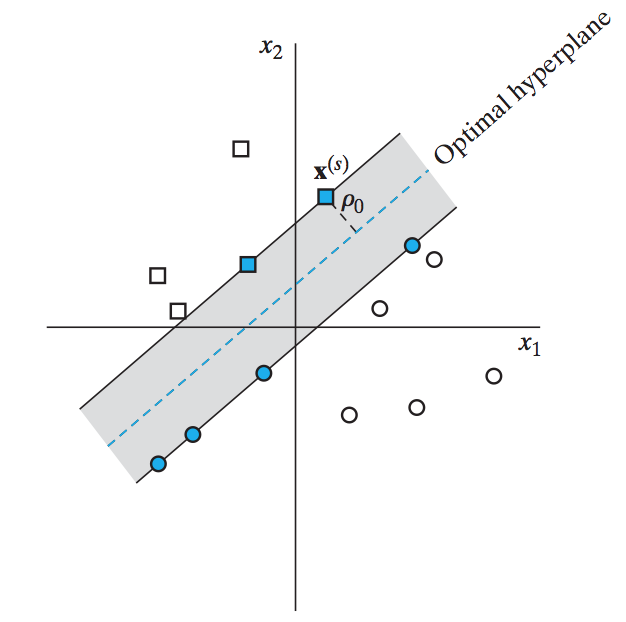
\includegraphics[scale=0.5]{images/support_vector}
\caption{Support Vectors}
\label{fig: support_vector}
\end{figure}
Therefore we want to find the maximum margin possible, defined in Equation \ref{eq: margin}.
\begin{equation}
g(x) = w x + b = \pm 1
\label{eq: discriminant}
\end{equation}
\begin{equation}
\begin{matrix}
r = \frac{g(x^{(2))}}{||w_o||} \\ 
\\
r =  \left  \{
 \begin{matrix}
  \frac{1}{||w_o||} \quad \text{if} \quad d^{(s)} = 1\\
  - \frac{1}{||w_o||} \quad \text{if} \quad d^{(s)} = -1 \\
  \end{matrix}	\\
\\
r = \frac{2}{||w_o||}
\end{matrix}
\label{eq: margin}
\end{equation}
Where $g(x)$ is the discriminant function, Equation \ref{eq: discriminant}, $x^(s)$ are the support vectors and $w_0$ is the  weight. Therefore, maximising the margin is equal to minimising $w_0$, so we can state our object function and the constrains, defined in Equation \ref{eq: hard_margin}. This is call \textbf{hard-margin}.
\begin{equation}
 \begin{array}{r c l}
	\text{min} \quad \Phi(w) = \frac{1}{2} w^Tw \\ 
	\\
	\text{subject to} \quad d_i(w_i^Tw_i + b_i) \ge 1 && \text{for} \quad 1 = 1,2, ..., N
\end{array}
\label{eq: hard_margin}
\end{equation}
This basic linear classifier can still be used to classify non-linear separable data by adding a set of non negative variables, $slacks$, $\{\epsilon\}_i^N$ in order to measure the deviation of the data from the ideal condition of pattern separability. Equation \ref{eq: softMargin} shows the updated equation, this method is called \textbf{soft margin}
\begin{equation}
 \begin{array}{r c l}
\text{min} \quad \Phi(w) = \frac{1}{2} w^Tw + c \sum_{k=0}^R \epsilon_k \\
	\\
\text{subject to} \quad d_i(w_i^Tw_i + b_i) \ge 1 - \epsilon_i && \epsilon_i > 0 \quad \text{for} \quad \text{all} \quad  i
\end{array}
\label{eq: softMargin}
\end{equation}
We skip the dual problems for simplicity, they are very simular to the non linear case only there is no \emph{kernel} and for the case of \emph{soft margin} the Lagrange multipliers must be also less than $C$. Thus we can express the optimal weight using this new information as follow:
\begin{equation}
w_o = \sum_{i=1}^{N(s)}\lambda_{0,j}d_ix_i^Tx^{(s)}
\label{eq: optimal_weight_lagrande}
\end{equation}
There $\lambda_{0,j}$ is a Lagrange multiplier.
\subsection{Non linear separable data}
As we stated before, a SVM maps from a linear input set to a non-linear \emph{feature set} using the  \emph{feature map} to infinite dimensional space, called \emp{feature space}, then it perform a linear map to the \emph{output state} . Figure \ref{fig: SVM} shows a graphical representation of a generic SVM
\begin{figure}[H]
\centering
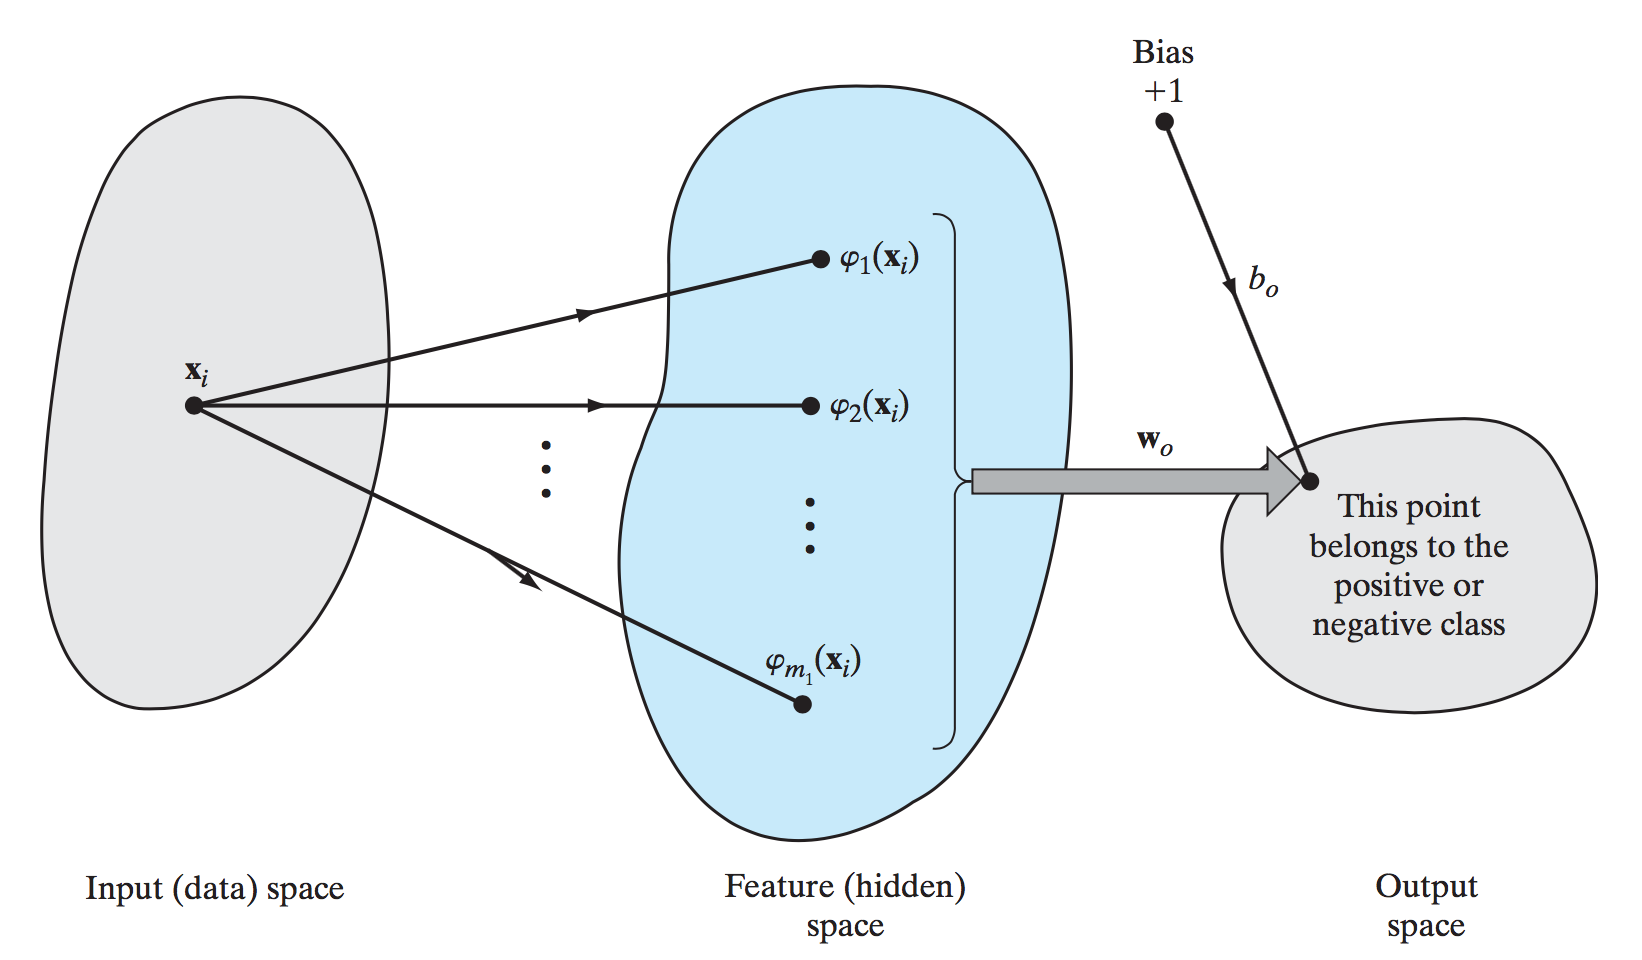
\includegraphics[scale=0.4]{images/SVM}
\caption{Mapping in a SVM}
\label{fig: SVM}
\end{figure}
Specifically, the \emph{feature map} is made by multiplying the inputs point with the \emph{feature vector}, a set of non linear function that transform , defined as follow:
\begin{equation}
\phi(x) = \{\varphi_j(x) \}^{\infty}_{j=1}
\label{eq: feature_map}
\end{equation}
Keeping in mind the Equation \ref{eq: optimal_hyperplane}, the optimal decise surface, we can re-state the optimal weight Equation \ref{eq: optimal_weight_lagrande} as follow:
\begin{equation}
w = \sum^{N^{(s)}}_{i = 1}a_id_i\phi(x_i)	
\end{equation}
Hence, substituting Equation \ref{eq: optimal_hyperplane}, we obtain
\begin{equation}
\sum^{N^{(s)}}_{i = 1}a_id_i\phi(x_i)^T\phi(x) = 0
\label{eq: optimal_hyperplane_feature}
\end{equation}
The term $\phi(x_i)^T\phi(x)$ represent a \emph{inner product}, let us denote it as the scalar:
\begin{equation}
\label{eq: kernel}
k(x, x_i) = \phi(x_i)^T\phi(x)  \\
= \sum^{\infty}_{j=1} \varphi_j(x_i)\varphi_j(x)
\end{equation}
The function $k(x, x_i)$ is called the \textbf{kernel}. According to this, we can re-express the optimal decise surface, Equation \ref{eq: optimal_hyperplane_feature}, by:
\begin{equation}
\sum^{N^{(s)}}_{i = 1}a_id_ik(x_i,x) = 0
\label{eq: optimal_hyperplane_feature}
\end{equation} 
Basically, the \textbf{kernel} computes the inner product of the images produced in the feature spaces under embedding $\phi$ of two data points in the input space. Equation \ref{eq: dual_problem_kernel} states the dual problem.
\begin{equation}
    \label{eq: dual_problem_kernel}
    \begin{aligned}
    \text{Maximixe } \lambda & \quad \sum^N_{i=1} \lambda_i - \frac{1}{2} \sum_{i=1}^N \sum_{j=1}^N \lambda_i \lambda_j d_i d_j k(x_i,x_j) \\
     \text{Subject to} & \\
           & \sum^N_{i=1} \lambda_i d_i = 0\quad \\
           & 0 \le \lambda_i \le C 
         \end{aligned}
    \end{equation}
The kernel must be decided \emph{a priori} from the user.
\section{Deep Learning}
\subsection{Supervised Learning}
In \textbf{supervised} learning there is a fixed training set consists on a set of example patterns and their targets. The objective is to learn a map between the inputs and the targets. 'Supervised' comes from the likeness between a student that tries to answer a question, and a teacher that knows the solution.

Therefore, at each step the algorithm can know how much wrong is prediction was, using a cost function, and it can improve it by applying a learning algorithm such as gradient descent in order to reduce the error.

\subsection{Reinforcement Learning}
In \textbf{reinforcement} learning the \emph{agent} takes \emph{actions} in an \emph{environment} in an to maximise a \emph{reward}. Figure \ref{fig: reinforcement_flow} shows the actions flow.

\begin{figure}[h]
\centering
	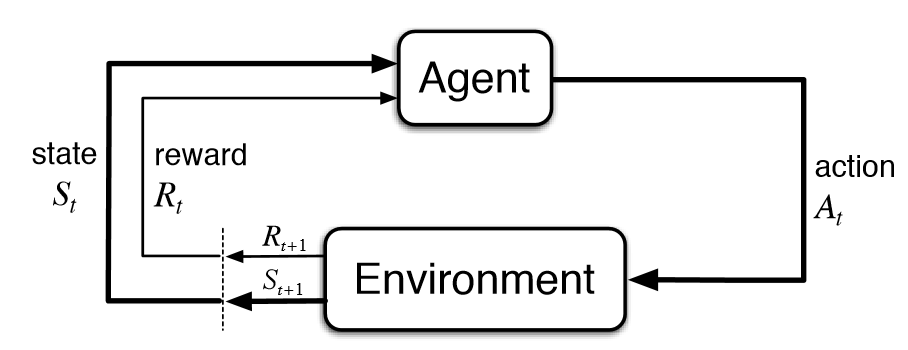
\includegraphics[scale=0.5]{images/reinforcement}
	\caption{Reinforcement Learning Flow}
	\label{fig: reinforcement_flow}
\end{figure}
\subsection{Unsupervised Learning}

\subsection{Training Techniques}
\subsubsection{Mini-batch}
\subsection{Regularisation}
\subsubsection{L1 Regularisation}
\subsubsection{Dropout Regularisation}
\subsection{Activations Functions}
\end{document}
